\section{Постановка задачи}
\label{sec:Chapter1} \index{Chapter1}

% \todo[inline]{Здесь надо максимально формально описать суть задачи, которую потребуется решить, так, чтобы можно было потом понять, в какой степени полученное в результате работы решение ей соответствует. Текст главы должен быть написан в стиле технического задания, т.е. содержать как описание задачи, так и некоторый набор требований к решению}

% (10-15 стр с картинками)
% (сюда то что мы не разрабатывали, а искали и использовали. в сожержательной именно то что я привнес в систему)

% \begin{enumerate}
%   \item 
%   \item 
%   \item 
%   \item 
%   \item 
%   \item 
% \end{enumerate}

\subsection{Требования для достижения цели работы}

Система должна:

\begin{itemize}
  \item Предоставлять возможность загрузки файлов на языке AlgoLoad в формате XML и автоматически преобразовывать их стандартную JSON структуру при помощи программного обеспечения в рамках общей системы визуализации графов алгоритмов.
  \item Преобразовывать промежуточные данные в интерактивную 3D модель графа алгоритма.
\end{itemize}

Решение описанных задач подразумевает многоэтапный процесс, который включает в себя:

\begin{itemize}
  \item Формирование архитектуры приложения и понятия внутреннего представления графа алгоритма. 
  \item Создание программного средства, преобразующего промежуточное представление графа алгоритма в JSON структуре в формат множества 3D моделей.
  \item Создание программного средства, производящего непосредственно интерактивную 3D визуализацию множества сформированных объектов, представляющих собой граф алгоритма. 
  \item Создание web-страницы, на которой производится визуализация и взаимодействие с интерфейсом.
\end{itemize}

\subsection{Требуемый формат входных данных}

Для работы системы требуется стандартизированное представление графа алгоритма. В данном случае исходным форматом данных для системы является JSON структура, содержащая информацию о координатах и типе вершин, и информацию о связанности этих вершин через их уникальные идентификаторы. Эта структура имеет следующий вид (пример из трех вершин и 2 дуг):

\begin{listing}[!ht]
\inputminted[frame=single,
             framesep=3mm,
             % linenos=true,
             % xleftmargin=21pt,
             tabsize=4]
            {js}{assets/json_file_example.json}
\caption{JSON структура, пример исходного формата данных}
\label{listing:json_file_example}
\end{listing}

\begin{figure}[!ht]
    \centering
    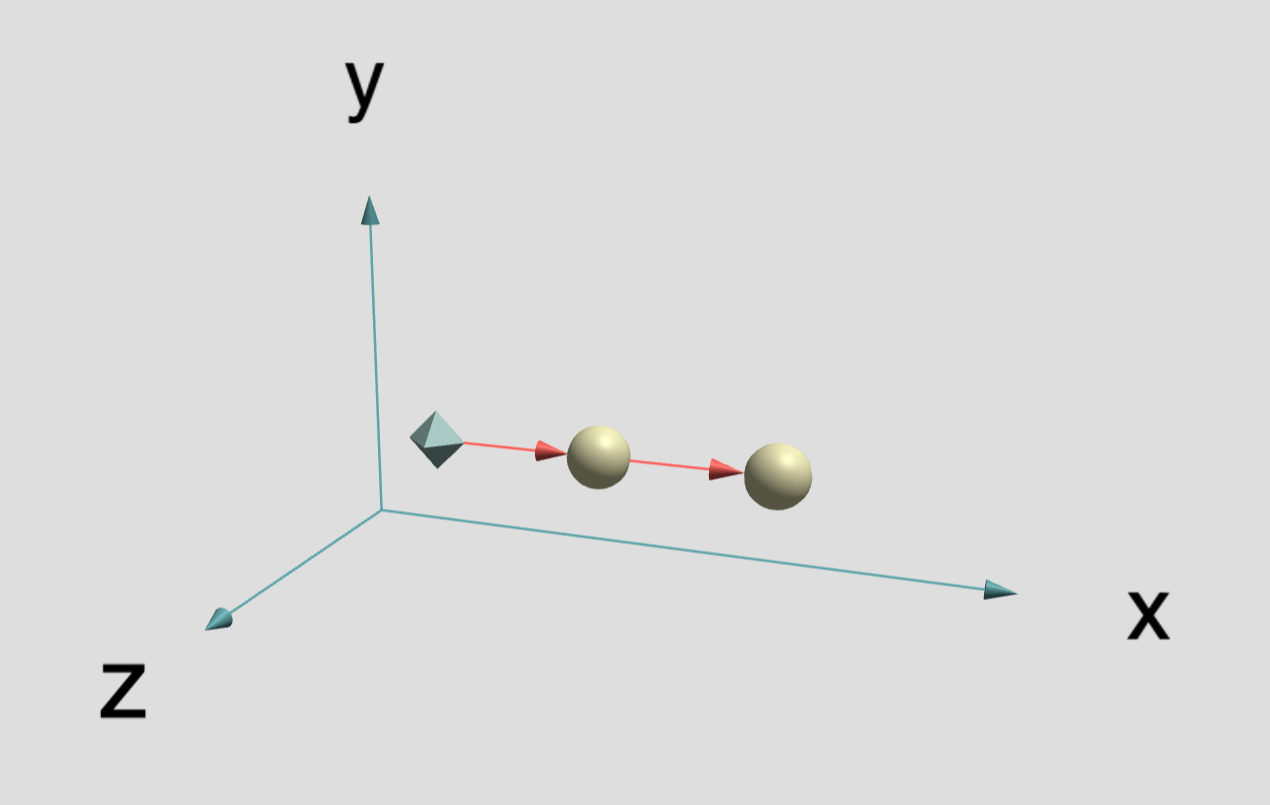
\includegraphics[width=0.9\textwidth]{assets/json_image.png}
    \caption{Пример визуализации графа, описанного в JSON структуре на listing \ref{listing:json_file_example}.}
    \label{fig:mesh1}
\end{figure}

% As you can see in the figure \ref{fig:mesh1}, the function grows near 0. Also, in the page \pageref{fig:mesh1} is the same example.

Набор данных, имеющийся в такой структуре выбран специально для рассматриваемой системы и в полной мере описывает граф алгоритма, который требуется визуализировать.


\subsection{Стандарт визуализации графов алгоритмов}

Стандарт визуализации графов алгоритмов - стандарт, впервые описанный как руководство, состоящее из набора правил, в соответствии с которыми рекомендуется изображать граф алгоритма. Существование стандарта обуславливается потребностью в построении изображений графов алгоритмов в общепринятом виде, который будет понятен вне зависимости от инструментов, используемых для изображения графа. \cite{AlgoWiki_standart}

Однако с появлением более универсального способа генерации изображений графов алгоритмов, такого как AlgoView, многие положения в стандарте требуется пересмотреть. Далее рассмотрим основные положения стандарта и некоторые изменения в нем, важные для составления требований к системе 3D визуализации. Нововведения в стандарте касаются автоматизации процесса и тем самым ослабления строгости требований к изображению графов.

\subsubsection{Требования к изображению графа алгоритма}

\begin{itemize}
    \item Визуализация алгоритма должна состоять минимум из одного изображения, трехмерной модели или проекции, содержащей граф алгоритма. Визуализация не дол-жна содержать графов, не имеющих отношения к описываемому алгоритму или графы, не соответствующие определению графа алгоритма.
    \item Граф алгоритма рекомендуется представлять для частного случая алгоритма и малого, фиксированного объема входных данных. Данный частный случай должен давать полное представление о структуре алгоритма.
\end{itemize}

\subsubsection{Оформление структуры графа алгоритма}

\begin{itemize}
    \item Вершины графа обозначаются геометрическими 3D объектами, вид, размер и цвет которых должен совпадать для всех операций одного вида. Вершины, соответствующие входным и выходным данным, отображаются иными геометрическими фигурами. Строгих правил в выборе вида вершин нет.
    \item Дуги графа обозначаются линиями со стрелками на концах, соответствующих "адресату" данных.
    \item Для изображения структуры требуется использовать трехмерную декартову систему координат, а также набор плоскостей, параллельных одной из координатных. На каждой плоскости вводится одинаковая равномерная сетка координат. Все вершины графа алгоритма располагаются на этих плоскостях в узлах сетки.
\end{itemize}

\subsection{Требования к 3D визуализации и возможностям анализа информационного графа}

Визуализация графа должна соответствовать нескольким требованиям:

\begin{itemize}
    \item Интерактивная визуализация должна работать в режиме реального времени на стандартном домашнем ПК и иметь интерфейс для взаимодействия с системой. Внешний вид интерфейса и графическая визуализация должны быть интуитивно понятны и удобны для работы при помощи компьютерной мыши и клавиатуры.
    \item Графическое представление графа должно содержать максимально возможное количество информации и соответствовать требованиям стандарта визуализации.
    \item Для удобного анализа требуется поддерживать разные настройки вида, такие как перспектива, проекция графа на плоскости, настройка осей координат. Настройки цветов и толщин линий, размер вершин. Все это влияет на удобство визуального анализа.
\end{itemize}
